\documentclass[hyperref=unicode]{beamer}

\usepackage[absolute,overlay]{textpos}
\usepackage{graphicx}
\usepackage{adjustbox}
\usepackage{mhchem}
\usepackage{wrapfig}
\usepackage{multirow}
\adjustboxset*{center}
\usepackage[utf8]{inputenc}
\usepackage{caption}

%dělení slov
\usepackage{ragged2e}
\let\raggedright=\RaggedRight
%konec dělení slov

\usepackage{fontspec}
\usepackage{unicode-math}

\usepackage{polyglossia}
\setdefaultlanguage{czech}

\def\uv#1{„#1“}

\mode<presentation>{\usetheme{Madrid}}
\DefineNamedColor{named}{pozadi}{RGB}{200,200,200}
\usecolortheme{crane}

\setbeamertemplate{footline}[frame number]

\addtobeamertemplate{frametitle}{
	\let\insertframetitle\insertsectionhead}{}
\addtobeamertemplate{frametitle}{
	\let\insertframesubtitle\insertsubsectionhead}{}

\makeatletter
\CheckCommand*\beamer@checkframetitle{\@ifnextchar\bgroup\beamer@inlineframetitle{}}
\renewcommand*\beamer@checkframetitle{\global\let\beamer@frametitle\relax\@ifnextchar\bgroup\beamer@inlineframetitle{}}
\makeatother
\setbeamercolor{section in toc}{fg=blue}
\setbeamertemplate{section in toc shaded}[default][100]

\usepackage{tikz}
\usetikzlibrary{positioning}
\usetikzlibrary{arrows}
\usetikzlibrary{shapes.multipart}

\title[Crisis]
{Koncentrace}

\subtitle{Směs, molární a molální koncentrace, hmotnostní a molární zlomek, směšovací rovnice, titrace}

%\author{\href{http://z-moravec.net/chemie/zaklady-chemie/}{http://z-moravec.net/}}

\date{}

\begin{document}

\frame{\titlepage}

\section{Směsi}
\frame{
	\begin{itemize}
	\item Směs je soustava, která obsahuje dvě nebo více chemických látek. Mezi složkami směsi nedochází k chemickým reakcím. Fyzikální vlastnosti (teplota varu, teplota tání, index lomu, atd.) směsi a~jednotlivých jejích složek jsou různé.
	\item Druhy směsí:
	\begin{itemize}
	\item heterogenní - lze rozeznat jednotlivé složky - suspenze, emulze, pěny, aerosoly
	\item homogenní - roztoky, slitiny
	\end{itemize}
	\item Koncentrace -- veličina popisující složení směsi.
	\end{itemize}
}

\section{Koncentrace}
\subsection{Molární a molální koncentrace}
\frame{
	\textbf{Molární koncentrace}
	\begin{itemize}
	\item Podíl látkového množství rozpuštěné látky a celkového objemu vzniklého roztoku.
	\item \ce{c = \frac{n}{V} = \frac{m}{MV} [mol.dm$^{-3}$ = M]}
	\end{itemize}
	\textbf{Molální koncentrace}
	\begin{itemize}
	\item Rozlišujeme hmotnostní a objemovou molalitu.
	\item Hmotnostní molalita je podíl látkového množství rozpuštěné látky a~hmotnosti rozpouštědla. Jednotkou je mol.kg$^{-1}$.
	\item \ce{$\mu$_A = \frac{n_A}{m_S} = \frac{m_A}{M_Am_S}}
	\item \textit{Objemová molalita} je podíl látkového množství rozpuštěné látky a~objemu rozpouštědla. Jednotkou je mol.dm$^{-3}$.
	\item \ce{$\mu'$_A = \frac{n_A}{V_S} = \frac{m_A}{M_AV_S}}
	\end{itemize}
}

\subsection{Hmotnostní zlomek}
\frame{
	\begin{itemize}
	\item Podíl hmotnosti složky a celkové hmotnosti roztoku.
	\item \ce{w_1 = \frac{m_1}{$\sum\limits_{i = 1}^n$ m_i}}
	\item Součet hmotnostních zlomků všech složek směsi je roven 1.
	\end{itemize}

	\textbf{Křížové pravidlo}

	$\begin{matrix}
	96 & & & & 45 \\
	& \searrow & & \nearrow &  \\
	& & 45 & & \\
	& \nearrow & & \searrow &  \\
	0 & & & & 51 \\
	\end{matrix}$

	Pro přípravu 45\% kyseliny sírové ředěním 96\% kyseliny vodou potřebujeme 45 hmotnostních dílů 96\% kyseliny a 51 hmotnostních dílů vody.
}

\subsection{Směšovací rovnice}
\frame{
	\begin{itemize}
	\item Popisuje slévání dvou a více roztoků, umožňuje spočítat koncentraci výsledného roztoku.
	\item $\sum\limits_{i=1}^n$ \ce{m_i w_i = mw}
	\item \ce{m_1w_1 +  m_2w_2 = mw}
	\item Pokud přidáváme čistou látku je w = 1.
	\item Pokud přidáváme rozpouštědlo je w = 0.
	\end{itemize}
	\vspace{3mm}
	\textbf{Příklad}

	Jaká je výsledná koncentrace roztoku vzniklého slitím 150 g 35 \% HCl a 200 cm$^3$ 15 \% HCl ($\rho_{15\%} = 1,073$ g.cm$^{-3}$)?
	\vspace{3mm}\\
	\ce{w = \frac{m_1.w_1 + V_2.$\rho$_{15\%}.w_2}{(m_1 +  V_2.$\rho$_{15\%})} = \frac{150.0,35 + 200.1,073.0,15}{(150 + 200.1,073)} = 0,23}
}

\subsection{Molární zlomek}
\frame{
	\begin{itemize}
	\item Podíl látkového množství složky směsi a celkového látkového množství všech složek ve směsi.
	\item \ce{X_1 = }$\frac{\textrm{n}_1}{\sum\limits_{i = 1}^n \textrm{n}_i}$
	\item $\sum\limits_{i=1}^n$ \ce{n_iX_i = 1}
	\item Součet molárních zlomků všech složek směsi je roven 1.
	\item Stejně jako v případě hmotnostního zlomku, jde o bezrozměrnou veličinu.
	\end{itemize}
}
\frame{
	\textbf{Příklad}

Spočítejte molární zlomky KBr a \ce{H2O} v 50,0~g roztoku o koncentraci 25~\% KBr.

m(KBr) = 12,5~g; n(KBr) = 0,11~mol\\[3mm]
m(\ce{H2O}) = 37,5~g; n(\ce{H2O}) = 2,08~mol
\ce{X(KBr) = \frac{0,11}{0,11 + 2,08} = 0,05}\\[3mm]
\ce{X(\ce{H2O}) = \frac{2,08}{0,11 + 2,08} = 0,95}\\[3mm]
\ce{X(\ce{H2O}) = 1 - X(KBr) = 0,95}
}

\section{Titrace}
\frame{
	\begin{columns}
	\begin{column}{0.6\textwidth}
	\begin{itemize}
		\item Koncentrace vzorku se zjišťuje pomocí reakce o odměrným roztok.
		\item Bod ekvivalence je zpravidla indikován barevnou změnou, ale lze použít i~instrumentální metody.
		\item Důležitou podmínkou je schopnost přesného odměřování objemů.
		\item Pro výpočet je nezbytné znát správně vyčíslenou rovnici reakce probíhající během titrace.
		\item Podle typu probíhající reakce rozlišujeme titrace:
		\begin{itemize}
			\item Neutralizační
			\item Srážecí
			\item Komplexotvorné
			\item Redoxní
		\end{itemize}
	\end{itemize}
	\end{column}
	\begin{column}{0.5\textwidth}
		\adjincludegraphics[width=\textwidth]{img/Titrace.jpg}
	\end{column}
	\end{columns}
}

\subsection{Sklo}
\frame{
	\begin{figure}
		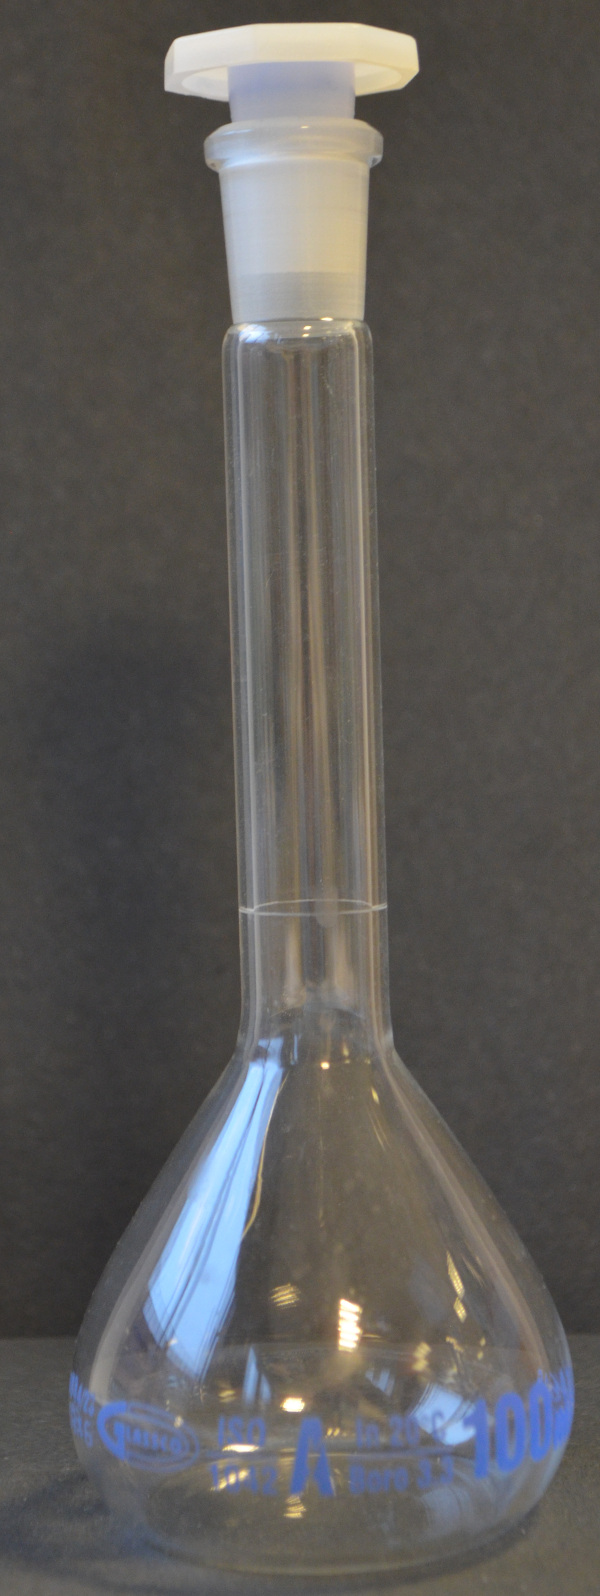
\includegraphics[height=0.7\textheight]{img/OdmBanka.jpg}
		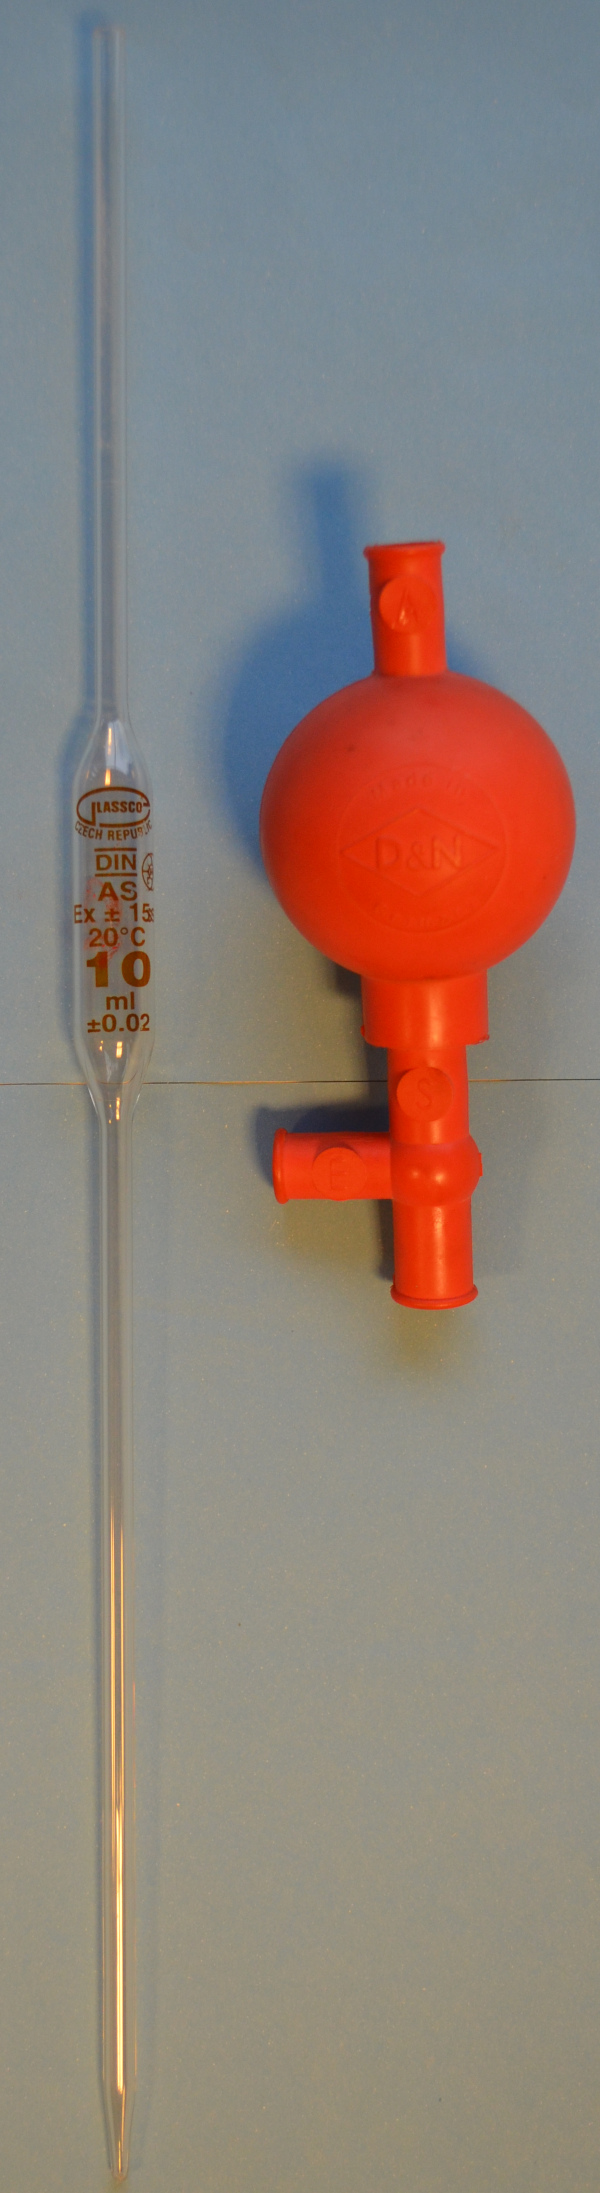
\includegraphics[height=0.7\textheight]{img/pipeta.jpg}
		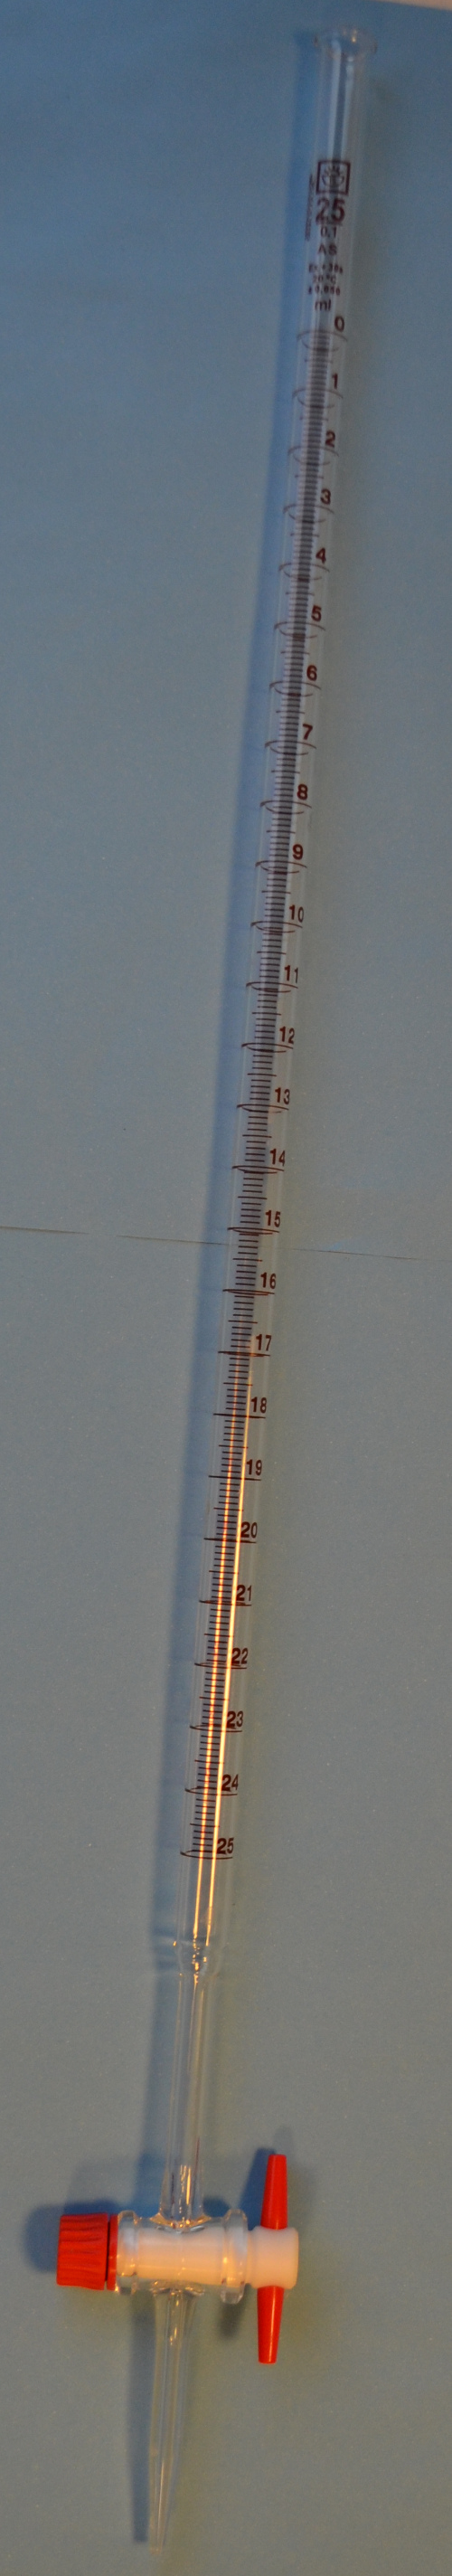
\includegraphics[height=0.7\textheight]{img/byreta.jpg}
		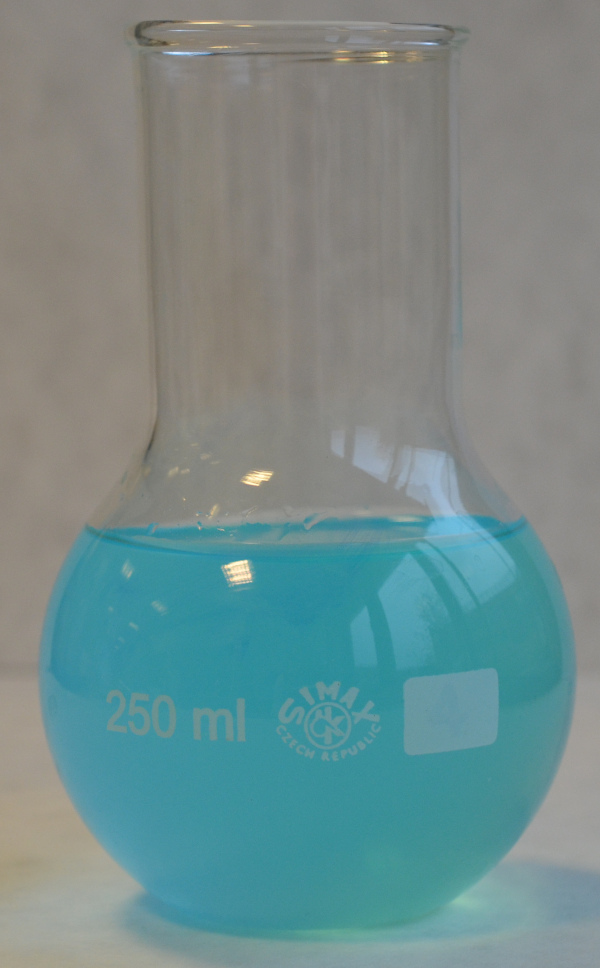
\includegraphics[height=0.7\textheight]{img/TitrBanka.jpg}
	\end{figure}
}

\subsection{Výpočet titrace}
\frame{
	\begin{itemize}
		\item Nutností je znát vyčíslenou rovnici.
		\item Titraci kyseliny sírové odměrným roztokem hydroxidu sodného můžeme popsat rovnicí:
		\item \ce{2 NaOH + H2SO4 -> Na2SO4 + 2 H2O}
		\item Látkové množství kyseliny sírové vypočítáme snadno:
		\item \ce{\frac{n(H_2SO_4)}{1} = \frac{n(NaOH)}{2}}
		\item \ce{n(H_2SO_4) = \frac{1}{2} $\cdot$ c(NaOH) $\cdot$ V(NaOH)}
		\item Koncentrace odměrného roztoku je zpravidla uvedena jako přibližná a je zpřesněna pomocí tzv. \textit{faktoru roztoku}. Např. roztok NaOH o koncentraci 0,1~M a faktoru 1,0125 má přesnou koncentraci:
		\item \ce{c = c_0 $\cdot$ f = 0,1 $\cdot$ 1,0125 = 0,1013}, vzorec pak můžeme upravit:
		\item \ce{n(H_2SO_4) = \frac{1}{2} $\cdot$ c(NaOH) $\cdot$ f(NaOH) $\cdot$ V(NaOH)}
	\end{itemize}
}

\frame{
	\begin{itemize}
		\item Druhým příkladem může být stanovení čistoty NaOH pomocí titrace odměrným roztokem HCl.
		\item \ce{NaOH + HCl -> NaCl + H2O}
		\item Navážka 0,4525 g NaOH byla rozpuštěna ve 100~cm$^3$ odměrné baňce, na titraci bylo odpipetováno 20~cm$^3$. Průměrná spotřeba činila 18,55~cm$^3$. Odměrný roztok HCl měl koncentraci 0,1~M a faktor 1,0583.
		\item Ve výpočtu musíme vzít v úvahu zřeďovací faktor. Z navážky jsme připravili 100~cm$^3$ roztoku, ale pro titraci jsme použili 20~cm$^3$.
		\item \ce{f_z = \frac{V(rozt)}{V(titr)} = \frac{100}{20} = 5}
	\end{itemize}
}

\frame{
	\begin{itemize}
		\item \ce{NaOH + HCl -> NaCl + H2O}
		\item n(NaOH) = n(HCl).f$_z$
		\item n(NaOH) = c(HCl).f(HCl).V(HCl).f$_z$
		\item m(NaOH) = c(HCl).f(HCl).V(HCl).f$_z$.M(NaOH)
		\item m(NaOH) = 0,1 . 1,0583 . 0,01855 . 5 . 40 = 0,393 g
		\item Čistotu NaOH pak spočítáme snadno:
		\item \ce{w = \frac{m(NaOH)}{m(nav)} = \frac{0,3926}{0,4525} = 0,867}
		\item \textbf{Čistota NaOH byla 86,7~\%.}
	\end{itemize}
}

\end{document}